% File ranlp2021.tex
%
%% Based on the style files for ACL-IJCNLP 2021, which were
%% Based on the style files for EMNLP 2020, which were
%% Based on the style files for ACL 2020, which were
%% Based on the style files for ACL 2018, NAACL 2018/19, which were
%% Based on the style files for ACL-2015, with some improvements
%%  taken from the NAACL-2016 style
%% Based on the style files for ACL-2014, which were, in turn,
%% based on ACL-2013, ACL-2012, ACL-2011, ACL-2010, ACL-IJCNLP-2009,
%% EACL-2009, IJCNLP-2008...
%% Based on the style files for EACL 2006 by
%%e.agirre@ehu.es or Sergi.Balari@uab.es
%% and that of ACL 08 by Joakim Nivre and Noah Smith

\documentclass[postprint]{flammie}

\usepackage{booktabs}
\usepackage{fancyvrb}
\usepackage{linguex}
\usepackage{graphics}


\title{Rules Ruling Neural Networks --- \\
Neural vs. Rule-Based Grammar Checking for a Low Resource
Language\footnotepubrights{find original in ACL anthology}}


\author{Linda Wiechetek\\
%$^\dagger$
UiT Norgga árktalaš\\
universitehta \\
Norway \\
  %\texttt{first.last@uit.no}
  \\\and{}
  Flammie A Pirinen \\ % $^\dagger$ \\
UiT Norgga árktalaš\\
universitehta \\  %Norway \\
Norway \\
  \\\and{}
  Mika Hämäläinen \\ %$^\ddagger$ \\
%  $^\ddagger$
University of Helsinki, \\
   Rootroo Ltd \\
  Finland\\
  %\texttt{first.last@helsinki.fi}
  \\\and{}
  Chiara Argese\\ % $^\dagger$ \\
UiT Norgga árktalaš\\
universitehta \\
Norway \\
}

\date{\today}

\begin{document}
\maketitle
\begin{abstract}

We investigate both rule-based and machine learning methods for the task of
compound error correction and evaluate their efficiency for North Sámi, a
low resource language.  The lack of error-free data needed for a neural
approach is a challenge to the development of these tools, which is not
shared by bigger languages. In order to compensate for that, we used a
rule-based grammar checker to remove erroneous sentences and insert compound
errors by splitting correct compounds.  We describe how we set up the error
detection rules, and how we train a bi-RNN based neural network.  The
precision of the rule-based model tested on a corpus with real errors
(81.0\%) is slightly better than the neural model (79.4\%). The rule-based
model is also more flexible with regard to fixing specific errors requested
by the user community. However, the neural model has a better recall (98\%).
The results suggest that an approach that combines the advantages of both
models would be desirable in the future. Our tools and data sets are
open-source and freely available on GitHub and Zenodo.
\end{abstract}

\section{Introduction}


This paper presents our work on automatically correcting compound errors in real
world text of North Sámi and exploring both rule-based and neural network
methods.  We chose this error type as it is the most frequent grammatical error
type (after spelling and punctuation errors) and twice as frequent as the second
most frequent grammatical error (agreement error). It also regards both spelling
and grammar as the error is a space between two words, but its correction
requires grammatical context.

A grammar checker is a writer's tool and particularly relevant to improve
writing skills of a minority language in a bilingual context, as is the case for
North Sámi.  According to UNESCO~\cite{moseley2010atlas}, North Sámi, spoken in
the North of Norway, Sweden and Finland, has around 30,000 speakers. It is a low
resource language in a bilingual setting, and language users frequently face
bigger challenges to writing proficiency as there is always a competing
language.~\cite{outakoski2015davvisamegielat} Developing a reliable grammar
checker with a high precision that at the same time covers a lot of errors has
therefore been our main focus.  Good precision (i.e.\ avoiding false alarms) is
a priority because users get easily frustrated if a grammar checker gives false
alarms and underlines correct sentences.



In this paper we focus on the correction of compound errors. This type of errors
is easy to generate artificially in the absence of large amounts of error
marked-up text, and we have a good amount of manually marked-up corpus for
evaluation for this error type.
Compound errors (i.e.\ one-word compounds that are erroneously written as two
words) can be automatically inserted by using a rule-based morphological
analyser on the corpus and splitting the word wherever we get a compound
analysis. Unlike other error types (like e.g.\ real word errors) they are easily
inserted, and existing compounds are seldom errors.  In addition, they are
interesting from a linguistic point of view as they are proper (complex)
syntactic errors and not just spelling errors and serve as an example for higher
level tools. Two adjacent words can either be syntactically related or erroneous
compounds, depending on the syntax.  In North Sámi orthography, as in the
majority languages spoken in the region (Norwegian, Swedish and Finnish), nouns
that form a new concept are usually written together. For example, the North
Sámi word \textit{boazodoalloguovlu} `reindeer herding area' consists of three
words \textit{boazu} `reindeer', \textit{doallu} `industry' and \textit{guovlu}
`area', and thus it is written together as a single compound. The task of our
methods is to correct spellings such as \textit{boazodoallu guovlu} into
\textit{boazodoalloguovlu} in case the words have been written  separately in
error.


We develop both a rule-based and a neural model for the correction of compound
errors. The rule-based model (\textit{GramDivvun})  is based on finite-state
technology and Constraint Grammar. The neural model is bi-directional recurrent
(BiRNN).  While the rule-based model has earlier produced good precision, it did
not handle unknown compounds well, which is why we were interested in a neural
approach.  However, neural models depend on  large amounts of `clean' data and
synthetic error generation (or alternatively marked-up data).


Typical for low-resource languages and also North Sámi, the corpora are not
clean and contain a fair amount of a variety of different spelling and
grammatical errors (see~\cite{antonsen2013callinmeattahusaid}).


Therefore, efficiently preparing data as to making it available for neural model
training is an important part of this paper.  In our case, we make  use of the
existing rule-based tools to both, generate synthetic error data and clean the
original data for training. For evaluation, on the other hand, we use real world
error data.

Our free and open-source rule-based tools can be found on GiellaLT
GitHub.\footnote{\url{https://github.com/giellalt/}} The training data and the
neural models are freely available on
Zenodo.\footnote{\url{https://zenodo.org/record/5172095}} We hereby want to
promote a wider academic interest in conducting NLP research for the North Sámi.

\section{Background}

Sámi open source rule-based language tools have a long and successful tradition
(nearly 20 years)~\cite{trosterud2004porting,
moshagen2011tilgjengelegheit,antonsen2011next,rueter2020fst}.
North Sámi is a low-resource language in terms of available corpus data (32.24M
tokens raw data). Although there is a fair amount of data, it contains many real
errors and only  a small amount is marked up for errors.


Applying neural approaches for high-level language tasks to low resource
languages is an interesting research question due the various limitations of
minority language corpora, versus the existing research in the topic in
well-resourced, majority languages and artificially constrained
setups~\cite{nekoto2020participatory}.  Rules have been used and are in a
wide-spread use in the context of endangered Uralic languages. There is recent
work on grammar checking for North Sámi~\cite{wiechetek2019seeing} and spell
checking for Skolt Sámi~\cite{trosterud2021soft}.  Other rule-based approaches
to grammar checking are extensively described in Wiechetek
\cite{wiechetek2017when}.

Before the era of neural models, it was common to use statistical machine
translation (SMT) as a method for grammar error
correction~\cite{behera2013automated,kunchukuttan2014tuning,
hoang2016exploiting}.  Many recent papers on grammar checking use bi-directional
LSTM models that are trained to tag errors in an input sentence. Such methods
have been proposed for Latvian~\cite{deksne2019bidirectional},
English~\cite{rei-yannakoudakis-2016-compositional} and
Chinese~\cite{huang2016bi}.  Similar LSTM based approaches have also been
applied for error
correction~\cite{yuan2016grammatical,ge2019automatic,jahan2021bangla}.  Other
recent approaches~\cite{kantor2019learning,omelianchuk2020gector} use methods
that take advantage of BERT~\cite{devlin-etal-2019-bert} and other data-hungry
models.  While such rich sentence embeddings can be used for English and a few
other languages with a large amount of data, their use is not viable for North
Sámi.

\section{Data}

For evaluation and training the neural model we use the \cite{sikor_06.11.2018}
(the Sámi International KORpus), which is a collection of texts in different
Sámi languages compiled by UiT The Arctic University of Norway and the Norwegian
Sámi Parliament. It consists of two subcorpora:
\textit{GT-Bound}\footnote{\url{https://gtsvn.uit.no/boundcorpus/orig/sme/}}
(texts limited by a copyright which are available only by request) and
\textit{GT-Free}\footnote{\url{https://gtsvn.uit.no/freecorpus/orig/sme/}} (the
publicly available texts). As a preprocessing step, we run a rule-based grammar
checker~\cite{wiechetek2012constraint} and remove sentences with potential compound
errors, as we cannot automatically ensure whether these errors are real or not.
This is needed as we want this data to be fully free of any compound errors as
it serves as the target side of our neural model.

Thereafter, we take in each sentence in this error free data and analyse it by a
rule-based morphological
analyser\footnote{\url{https://github.com/giellalt/lang-sme}}. When the analyser
sees a potential compound word, it indicates the word boundary with a compound
(\texttt{+Cmp\#}) tag. We use this information to automatically split all
compounds identified by the rule-based analyser. This results in a parallel
corpus of the original sentences as the prediction target and their
corresponding versions with synthetically introduced compound errors. Many of
the compound boundaries are ambiguous, and the algorithm decides the one used in
training data based on heuristics: maximum number of compound boundaries where
the splitting will not cause any other modifications of the word stems or other
content.

As an additional data source, we use the North Sámi Universal Dependencies
treebank~\cite{tyers-sheyanova-2017-annotation}. We parse the corpus with
UralicNLP~\cite{uralicnlp} and split the compounds the rule-based
morphological analyser identifies as consisting of two or more words in order to
synthetically introduce errors.  We also run the rule-based morphological
analyser and morpho-syntactic disambiguator to add  \textit{part-of-speech}
(POS) information to produce an additional data set with POS tags. For the
Universal Dependencies data, we use the POS tags provided in the data set.

We then make sure that all sentences have at least one generated compound error
and that the only type of error the sentences have is the compound error (no
other changes introduced by the rule-based models). We shuffle this data
randomly and split it on a sentence level into 70~\% training, 15~\% validation
and 15~\% testing. The size of the data set can be seen in
Table~\ref{tab:data-stats}, the sentences were tokenized based on punctuation
marks.

\begin{table}[htb]
\centering \small
\begin{tabular}{lcc}
\toprule
           & \textbf{Sentences} & \textbf{Source tokens} \\ \midrule
\textbf{Train}      & 43,658    & 388,167       \\
\textbf{Test}       & 9,356     & 83,107        \\
\textbf{Validation} & 9,355     & 82,566        \\
\midrule
\textbf{Real-world errors} & 3,291 & 26,565 \\
\bottomrule
\end{tabular}
\caption{Training, testing and validation sizes for the \textbf{neural model}
    (corpus with synthetic errors)\label{tab:data-stats}}
\end{table}

For the rule-based model \textit{GramDivvun} we do not generate synthetic
errors. We have hand-selected a large corpus for rule development and as
regression tests, consisting of representative sentences from \textit{GT-Free}.
The current selection for syntactic compound errors includes 3,291 sentences
with real world compound errors (and possibly other errors in addition).

\section{Methods}

We use a neural models and a rule-based model for compound error  correction.

\subsection{Neural Model}

\begin{table*}[htb]
\centering
\begin{tabular}{|l|l|p{6.5cm}|}
\hline
\textbf{n} & \textbf{Input}                                                                                                                                                                                                                                                                 & \textbf{Output}                                                                   \\ \hline
2 & g e a h č č a l a d d a n \_ p r o š e a k t a n                                                                                                                                                                                                                      & g e a h č č a l a d d a n p r o š e a k t a n                            \\ \hline
3 & g e a h č č a l a d d a n \_ p r o š e a k t a n \_ p r o š e a k t a n                                                                                                                                                                                               & g e a h č č a l a d d a n p r o š e a k t a n \_ p r o š e a k t a n     \\ \hline
2 & V\textgreater~g e a h č č a l a d d a n \textless{}V \_ N\textgreater~p r o š e a k t a n \textless{}N                                                                                                                                                                & g e a h č č a l a d d a n p r o š e a k t a n                            \\ \hline
3 & \begin{tabular}[c]{@{}l@{}}V\textgreater~g e a h č č a l a d d a n \textless{}V \_ N\textgreater~p r o š e a k t a n \textless{}N \_ \\ N\textgreater~j a g i \textless{}N\end{tabular}                                                                               & g e a h č č a l a d d a n p r o š e a k t a n \_ p r o š e a k t a n     \\ \hline
\end{tabular}
\caption{Examples of the character-level input and output, where \textit{n}
    indicates the chunk size. The first examples are without POS tags and the
    last with POS tags\label{tab:example-input-output}}
\end{table*}

We model the problem at a character instead of word level in NMT (neural machine
translation). The reason for using a character-level model instead of a
word-level model is that, this way, the model can work better with
out-of-vocabulary words. This is important due to the low-resourced nature of
North Sámi, although there are other deep learning methods for endangered
languages that do not utilize character level models~\cite{alnajjar2021when}. In
practice, we split words into characters separated by white spaces and mark
actual spaces between words with an underscore (\_).  We train the model to
predict from text with compound errors into text without compound errors. As
previous research~\cite{partanen-etal-2019-dialect,alnajjar2020automated} has
found that using chunks of words instead of full sentences at a time improves
the results in character level models, we will be training different models with
different chunk sizes.  This means that we will train a model to predict two
words at a time, three words at a time, all the way to five words at a time.

We train the models with and without POS tags. For the models with POS tags, we
surround each word with a token indicating the beginning and the end of the POS
tag. The POS tags are included only on the source side, not on the target side.
They are separated from the word with a white space.

An example of the data can be seen in Table~\ref{tab:example-input-output}. Even
though every sentence in the training data has a compound error, this does not
mean that every input chunk the model sees would have a compound error. This
way, the model will also learn to leave the input unchanged if no compound
errors are detected.

We train all models using a bi-directional long short-term memory (LSTM) based
model~\cite{hochreiter1997long} by using OpenNMT-py~\cite{opennmt} with the
default settings except for the encoder where we use a
BiRNN~\cite{schuster1997bidirectional} instead of the default RNN (recurrent
neural network), since BiRNN based models have been shown to provide better
results in character-level models~\cite{hamalainen2019revisiting}.  We use the
default of two layers for both the encoder and the decoder and the default
attention model, which is the general global attention presented by
\cite{luong2015effective}.  The models are trained for the default of 100,000
steps. All models are trained with the same random seed (3,435) to ensure
reproducibility.

During the training of the neural models, we evaluate the models using simple
sentence level scores. There we look only at full-sentence matches and evaluate
their accuracy, precision and recall, as opposed to the evaluations in
Section~\ref{sec:evaluation}, where we study them more carefully at the
word-level.  The results of the neural models for the generated corpus (where
errors were introduced by splitting compounds) can be seen in
Table~\ref{tab:results-neural}. The results indicate that both of the models
receiving a chunk of two words at a time reached to the highest accuracy, and
the model without the POS tags also reached to the highest precision.

\begin{table}[htb]
\centering
\begin{tabular}{lllll}
\toprule
\bf Chunk & \bf POS & \bf Accuracy            & \bf Precision           & \bf
    Recall         \\ \midrule
2     & no  & \textbf{0.925} & \textbf{0.949} & 0.974          \\
3     & no  & 0.847          & 0.883          & 0.955          \\
4     & no  & 0.852          & 0.892          & 0.950          \\
5     & no  & 0.869          & 0.909          & 0.952          \\
2     & yes & \textbf{0.925} & 0.948          & \textbf{0.976}          \\
3     & yes & 0.906          & 0.934          & 0.968          \\
4     & yes & 0.856          & 0.896          & 0.951 \\
5     & yes & 0.857          & 0.895          & 0.953          \\
    \bottomrule
\end{tabular}
\caption{Sentence level scores for different neural models tested on a corpus
    with artificially introduced errors\label{tab:results-neural}}
\end{table}


The POS tags were not important for the models, as the results with and without
them are fairly similar. The largest gain was when the compound error correction
was done for three words at a time. As this performance gain only occurred for
that specific model, it suggests that it is more of an artefact of the training
data and how it is fed into the model than any actual improvement.



\subsection{Rule-based Model}

The rule-based grammar checker \textit{GramDivvun} is a full-fledged grammar
checker fixing spelling errors, (morpho)-syntactic errors (including real word
spelling errors\footnote{Real word errors are spelling errors where the outcome
is an actual word that is not fit for the context.}, inflection errors, and
compounding errors) and punctuation and spacing errors.


It takes input from the finite-state transducer (\textit{FST}) to a number of
other modules, the core of which are several Constraint Grammar modules for
tokenization disambiguation, morpho-syntactic disambiguation and a module for
error detection and correction. The full modular structure
(Figure~\ref{fig:my_label}) is described in
Wiechetek~\cite{wiechetek2019seeing}.  This work regards  predominantly the
modification of the disambiguation and error detection modules
\textit{mwe-dis.cg3}, \textit{grc-disambiguator.cg3}, and
\textit{grammerchecker-release.cg3}.  We are using finite-state
morphology~\cite{beesley2003finite} to model word formation processes.  The
technology behind our \textit{FSTs} is described in
Pirinen~\cite{pirinen2010finitestate}.  Constraint Grammar is a rule-based
formalism for writing disambiguation and syntactic annotation
grammars~\cite{karlsson1990constraint,karlsson1995constraint}.  In our work, we
use the free open source implementation VISLCG-3~\cite{didriksen2015cg3}. All
components are compiled and built using the \textit{GiellaLT}
infrastructure~\cite{moshagen-etal-2013-building}.  The code and data for the
model is available for
download~\footnote{\url{https://github.com/giellalt/lang-sme/releases/tag/naacl-2021-ws}}
with specific version tagged for reproducibility.


    \begin{figure*}[ht]
    \begin{center}
    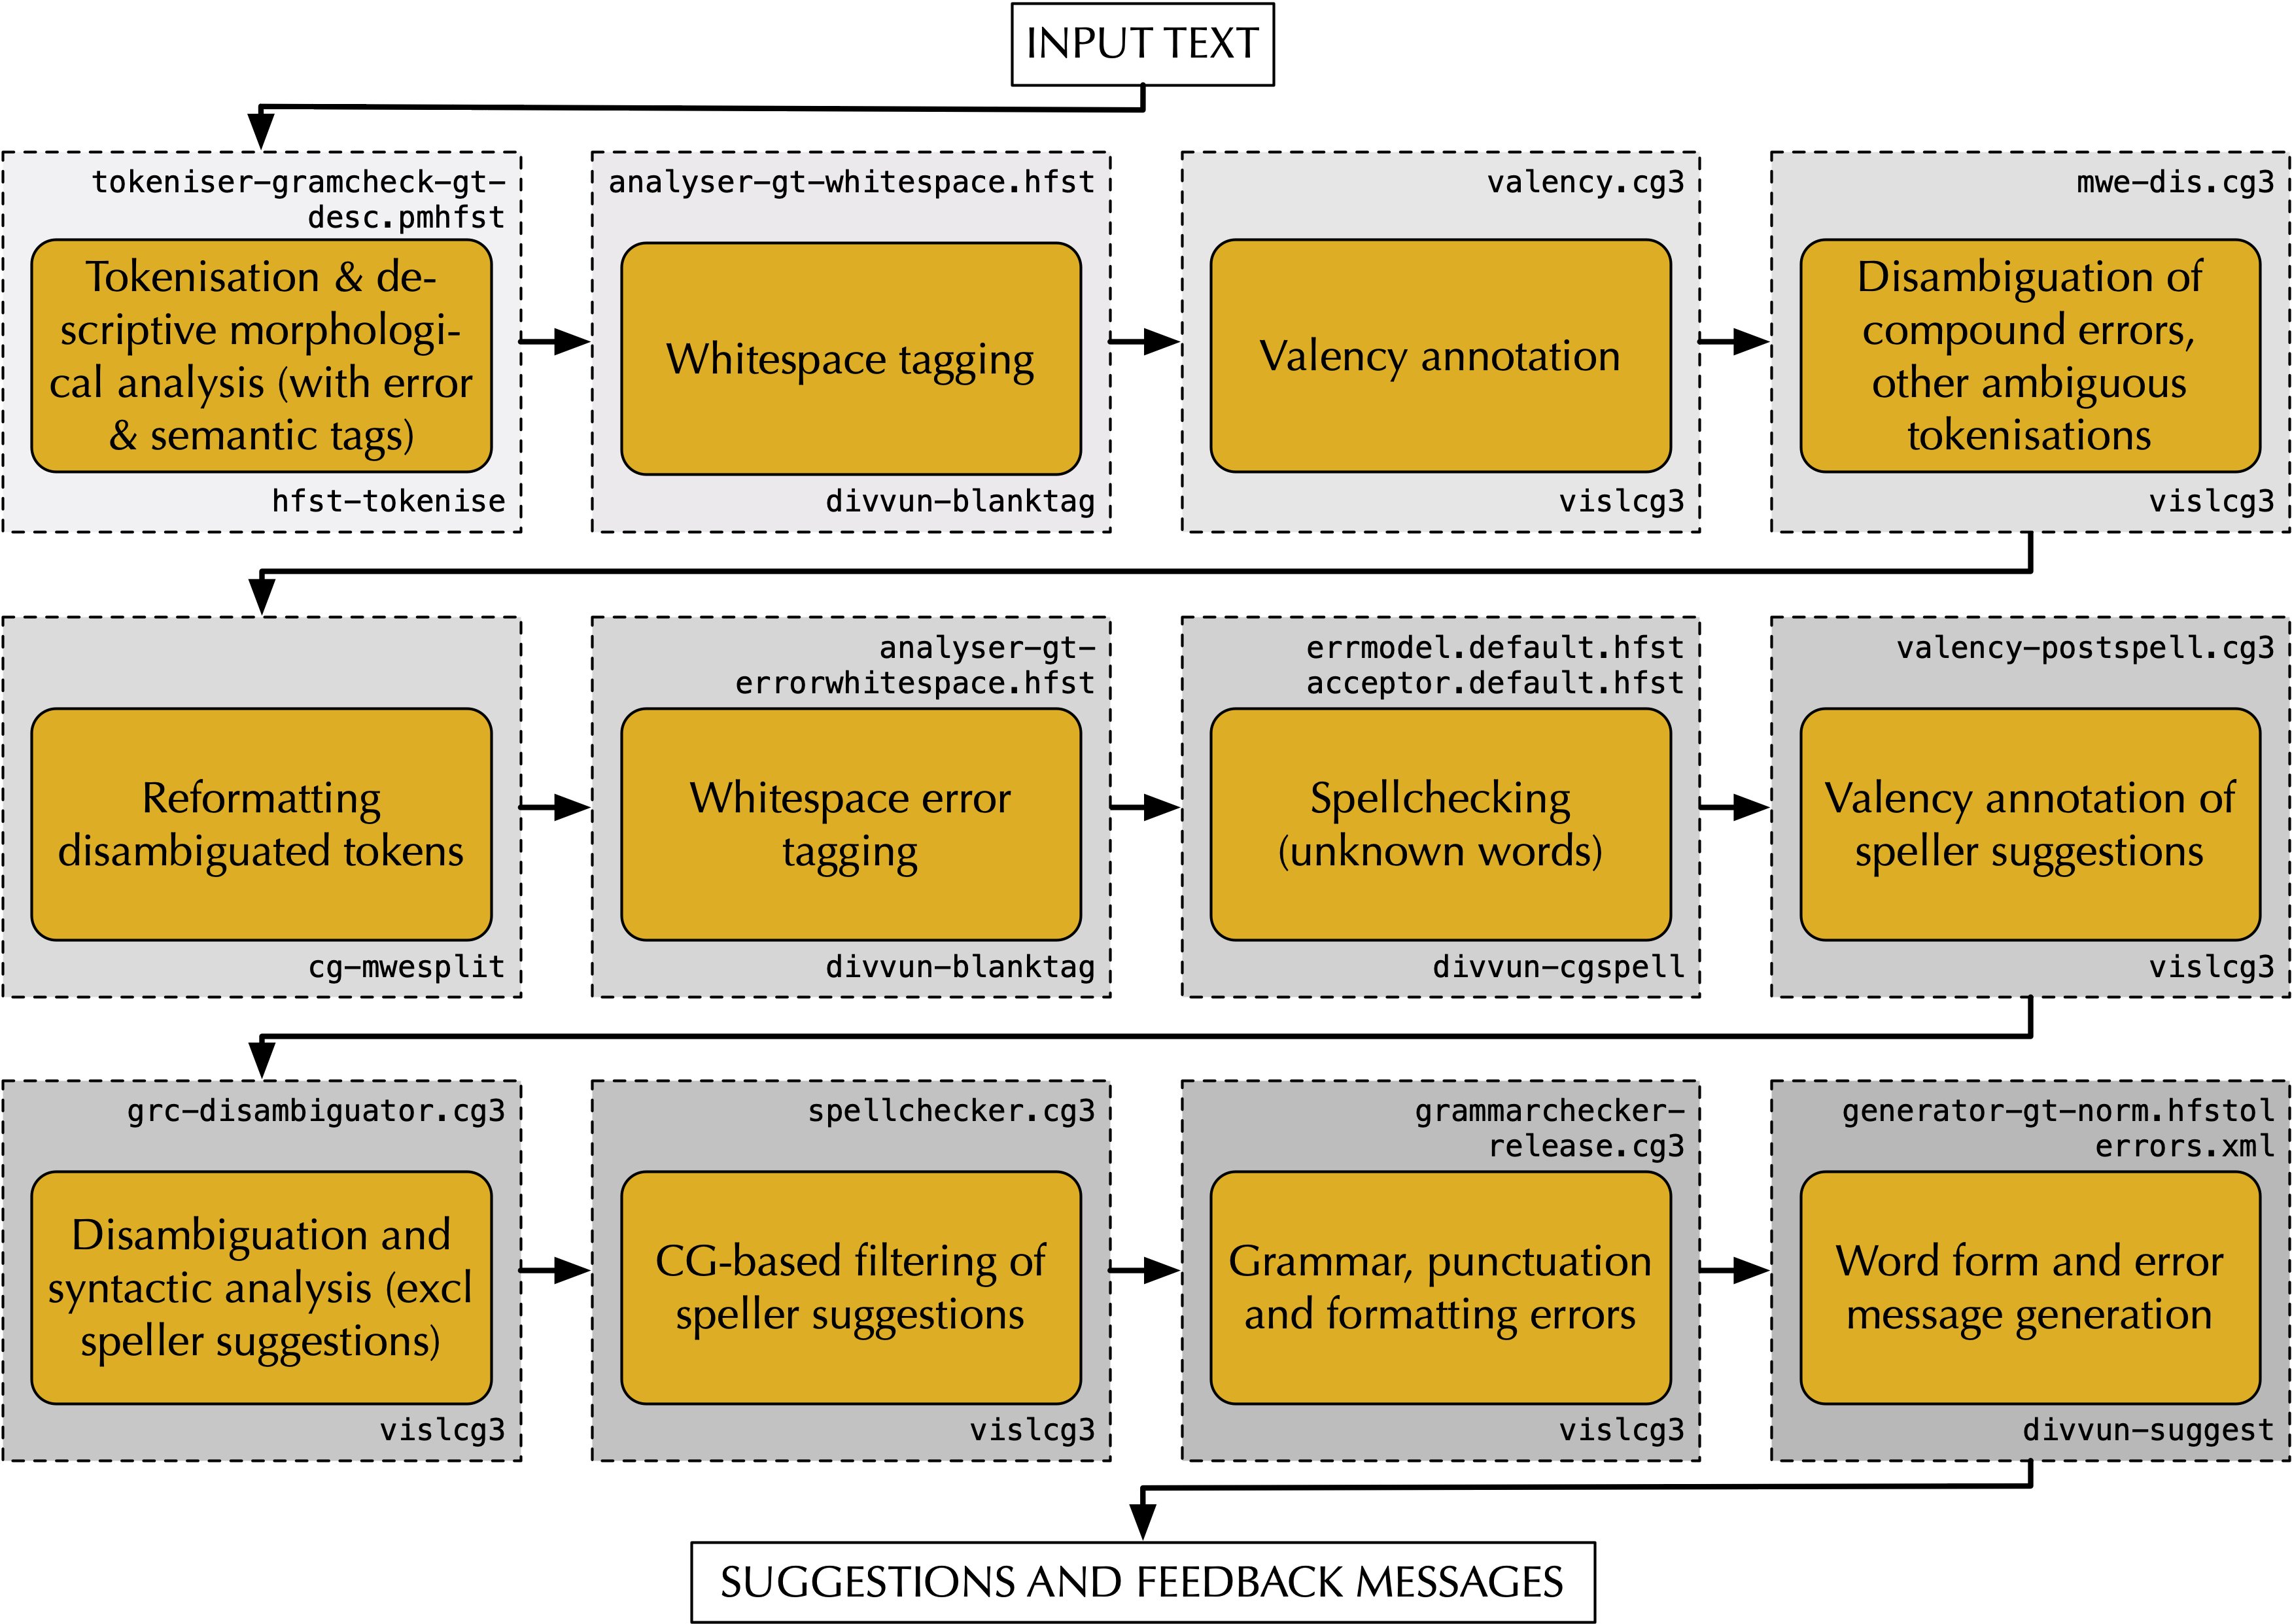
\includegraphics{GramCheckLightFlow-08-2021.png}
    \caption{System architecture of the North Sámi grammar checker
        (\textit{GramDivvun})\label{fig:my_label}}
    \end{center}
    \end{figure*}


The syntactic context is specified in hand-written Constraint Grammar rules. The
REMOVE-rule below removes the compound error reading (identified by the tag
\texttt{Err/SpaceCmp}) if the head is a 3rd person singular verb (cf.\ l.2) and
the first element of the potential compound is a noun in nominative case (cf.\
l.3). The context condition further specifies that there should be a finite verb
(VFIN) somewhere in the sentence (cf.\ l.4) for the rule to apply.

\begin{Verbatim}[frame=single,framerule=0.2mm,framesep=3mm,fontsize=\footnotesize,baselinestretch=1]
REMOVE (Err/SpaceCmp)
(0/0 (V Sg3))
(0/1 (N Sg Nom))
(*0 VFIN);
\end{Verbatim}


All possible compounds written apart are considered to be errors by default,
unless the lexicon specifies a two or several word compound or a syntactic rule
removes the error reading.

The process of rule writing includes several consecutive steps, and like neural
network models they require data. The process is as follows:

\begin{enumerate}
    \item Modelling an error detection rule based on at least one actual
        sentence containing the error
    \item Adding constraints based on the linguist's knowledge of possible
        contexts (remembered data)
    \item A corpus search for sentences containing similar forms/errors, testing
        of the rule and reporting rule mistakes
    \item Modification of constraints in the rule based on this data and testing
        against regression tests so that unfit constraints depending on results
        for precision and recall (focus on precision)
\end{enumerate}

The basis of rule development is continuous integration. Typical shortcomings
and bad errors can be fixed right away with added conditions. Neural models are
not usually trained in this way.

The frequent experience of false alarms can decrease the users' trust in the
grammar checker.  Typically, full-fledged user oriented grammar checkers, e.g.
\textit{DanProof} focus on keeping false alarms low and precision
high~\cite{bick2015danproof} because users' experiences have shown that certain
experiences will frustrate users and stop them from using the application.

For rule development, regression tests are used. These consist in error-specific
YAML\footnote{\url{https://yaml.org/spec/1.2/spec.html}} tests and are manually
marked up.

The regression test for compound errors contains 3,291 sentences (1,368 compound
errors, used for development and regression) give the results as shown in
Table~\ref{tab:rule_based_res}.


\begin{table}[htb]
    \centering
    \begin{tabular}{lll}
    \toprule
        \bf Precision & \bf Recall & \bf $F_1$ score \\
        \midrule
        94.95 & 86.22 & 90.80 \\
        \bottomrule
    \end{tabular}
    \caption{The \textbf{rule-based model} tested on the developer's corpus
    (regression tests)\label{tab:rule_based_res}}
\end{table}




\section{Results}\label{sec:evaluation}

We evaluate the models both quantitatively and qualitatively.  We evaluate on
accuracy, precision and recall, and do a linguistic evaluation.  The
measurements are defined in this article as follows: Accuracy $A = \frac{C}{S}$,
where C is a correct sentence (1:1 string match) and $S$ is corpus size in
sentences, precision $P = \frac{tp}{tp + fp}$ and recall $R = \frac{tp}{tp +
fn}$, where $tp$ is true positive, $fp$ is false positive and $fn$ is false
negative.  The $F_1$ score is the harmonic mean of precision and recall $F_1 = 2
\times \frac{P \times R}{P + R}$. The accuracy is thus sentence level
correctness rate---as used in the method section to probe model
qualities---whereas precision measures how often corrections were right and
recall measures how many errors we found.  The word-level errors are counted
once per error in the marked-up corpus. Thus, if a three-part compound contains
two compounding errors it is counted towards the total as one error, but if a
sentence has three separate compounds with wrong splits each, we count three
errors.


The error marked-up corpus we used includes 140 syntactic compound errors (there
are other compound errors that can be discovered by the spellchecker as they are
word internal) and is from \textit{GT-Bound}. We chose \textit{GT-Bound} to make
sure that the sentences had not been used to develop rules. It is part of our
error-marked up corpus, which makes it possible to run an automatic analysis.
This error corpus does only contain real world (as opposed to synthetic)
errors.

\begin{table}[htb]
\centering
\begin{tabular}{lllll}
\toprule
\textbf{Chunk} & \textbf{POS} & \textbf{Accuracy}   & \textbf{Precision}  &
    \textbf{Recall} \\ \midrule
2     & no  & \textbf{0.781} & \textbf{0.794} & \textbf{0.980}  \\
3     & no  & 0.707 & 0.720 & 0.974  \\
4     & no  & 0.726 & 0.747 & 0.963  \\
5     & no  & 0.727 & 0.757 & 0.950  \\
2     & yes & 0.777 & 0.788 & 0.982  \\
3     & yes & 0.761 & 0.775 & 0.976  \\
4     & yes & 0.720 & 0.744 & 0.958  \\
5     & yes & 0.751 & 0.765 & 0.976  \\
    \bottomrule
\end{tabular}
\caption{Sentence level scores for the neural models tested on a real world
    error corpus\label{tab:neural-real-world-res}}
\end{table}

Table~\ref{tab:neural-real-world-res} shows the results for the neural models on
this corpus. The drop in results is expected as the models were trained on
synthetic data, whereas this data consists of real world errors. However, the
results stay relatively good, given that synthetic data was the only way to
produce enough training data for North Sámi.

We ran the neural and rule-based model on two different corpora of compound
error materials, i.e.\ synthetic and real world.  Table~\ref{tab:my_label} shows
the evaluation on a real world error corpus.

\begin{table}[htb]
    \centering
    \begin{tabular}{lrrr}
    \toprule
        \bf Model & \bf Precision & \bf Recall & \bf $F_1$ \\
        \midrule
        Rule-based model & 81.0 & 60.7 & 69.3 \\
        Neural model & 79.4 & 98.0 & 87.7 \\
        \bottomrule
    \end{tabular}
    \caption{Results for \textbf{both models} based on a manually marked-up
    evaluation corpus\label{tab:my_label}}
\end{table}


The neural network performs well in terms of numbers, but has the following
shortcomings that are  problematic for the end users.  It introduces new (types
of) errors unrelated to compounding, like changing \textit{km²} randomly either
to \textit{kmy} or \textit{km} kind of unforgivable (because not understandable)
for the end user.  They introduce compounds like \textit{Statoileamiálbmogiid}
`Statoil (national oil company and gasstation) indigenous people' as in
ex.~\ref{statoil}.  The rule-based grammar checker presupposes that the compound
is listed in the lexicon, which is why these corrections can easily be avoided.

\exg. \textbf{Statoil} \textbf{eamiálbmogiid} eatnamiid billisteami birra\label{statoil}\\
Statoil indigenous.people.\textsc{acc.pl} land.\textsc{acc.pl} destruction\textsc{.gen} about\\
`about the destruction of the indigenous peoples' territories by Statoil'


It also produces untypically long non-sense words like
\textit{NorggaSámiidRiidRiidRiidRiidRiidRiidRiikasearvvi}.  In addition, there
are false positives of certain grammatical combinations that are systematically
avoided by rule-based grammar checker.  These are combinations of attributive
adjectives and nouns (17 occurrences) like \textit{boares eallinoainnuid} in
ex.~\ref{boareseallinoainnuid} and genitive modifier and noun combinations (11
occurrences) like \textit{njealjehaskilomehtera eatnamat} in
ex.~\ref{njealjehas}.

\exg. \textbf{boares} \textbf{eallinoainnuid} ja modearna servodaga váikkuhusaid gaskii.\label{boareseallinoainnuid}\\
old life.view\textsc{.acc.pl} and modern society\textsc{.gen} impact\textsc{.acc.pl} between \\
`between old philosophies and the impact of modern society'

\exg. Dasalassin 137000 \textbf{njealjehaskilomehtera} \textbf{eatnamat} biđgejuvvojit seismalaš linnjáid\label{njealjehas}\\
in.addition 137000 square.kilometre\textsc{.gen} land\textsc{pl.} split\textsc{.pass.pl3} seismic line\textsc{.acc.pl} \\
`In addition, 137,000 square kilometres of land are split by seismic lines'


The rule-based model, on the other hand, typically suggests compounding, where
both compounding and two word combinations would be adequate, for example in the
case of the first part of the compound having homonymous genitive and a
nominative analyses. The suggested compound is not an error. However, the
written form is grammatically correct as well. These suggestions still count as
false positives. Other typical errors are cases where there are two accepted
ways of spelling a compound/MWE as in ex.~\ref{ridduriddu}, where both
\textit{Riddu Riđđu} and \textit{Riddu-Riđđu} are correct spellings, and the
latter one is suggested as a correction of the former one.

\exg. ovdanbuktojuvvojit omd. jahkásaš \textbf{Riddu Riđđu} festiválas.\label{ridduriddu}\\
present\textsc{.pass.prs.pl3} e.g. annual {Riddu Riđđu} festival\textsc{.loc}\\
`they are presented at the annual Riddu Riđđu festival.

The rule-based model also struggles predominantly with false negatives, like
\textit{njunuš olbmot} `leading people' that are due to missing entries in the
lexicon like in ex.~\ref{njunus}.

\exg. Sii leat gieldda \textbf{njunuš} \textbf{olbmot}.\label{njunus}\\
they are municipality\textsc{.gen} leading people\\
`They are the leading people of the municipality'



\section{Discussion}


In the future, we would like to look into hybrid grammar checking of other error
types and other (Sámi) languages.

The neural approach gives us relatively high recall in the real world situation
with lower precision, whereas the rule-based model is designed to give us high
precision even at the cost of lower recall (user experience), which is why
hybrid approaches that combine the best of two worlds are interesting.


Noisy data is to be expected in any endangered language context, as the language
norms are to a lesser degree internalized.  We will therefore need a way of
preparing the data to train neural networks, which can either consist in
creating synthetic data or automatically fixing errors and creating a parallel
corpus.

When creating synthetic data for neural networks, the amount of data is hardly
the main issue. Many generative systems are capable of over-generating data. The
main question that arises is the quality and representatives
(\cite{hamalainen2019template}) of the generated data. If the rules used to
generate the data are not in line with the real world phenomenon the neural
model is meant to solve, we cannot expect very high quality results in real
world data.

Generated sentences can easily be less complex `text book examples' that are not
representative of real world examples.  In the case of agreement errors between
subjects and verbs, for example, there are long distance relationships and
complex coordinated subjects including personal pronouns that can change the
structure of a seemingly straightforward relation.  Therefore, we advocate the
use of high quality rule-based tools  to prepare the data, i.e.\ fix the errors
and create a parallel corpus.

While synthetic error data generation for compound errors is somewhat more
straightforward as it only affects adjacent words, the generation of synthetic
error corpora for other error types is not as straightforward, in part also
because generating synthetic errors of other kind can potentially create valid
and grammatically correct sentences with different meanings.  We therefore
predict that (hybrid) neural network approaches for other error types that
either involve specific morphological forms (of which there are many in North
Sámi) or changes in word order will be more difficult to resolve.





\section{Conclusion}




In this paper, we have developed both a neural network and a rule-based grammar
checker module for compound errors in North Sámi.  We have shown that a neural
compound-corrector for a low-resource language can be built based on synthetic
error data by introducing the compound errors using a high level rule-based
grammar models.  It is based on the rule-based tools to both generate errors and
clean the data using both part-of-speech analysis, disambiguation and even the
error detector.

The rule-based module is embedded in the full-fledged \textit{GramDivvun}
grammar checker and achieves a good precision of 81\% and a lower recall of
61\%. A higher precision, even at  the cost of a lower recall, is in line with
our objective of keeping false alarms low, so users will be comfortable using
our language tools.  The neural network achieves a slightly lower precision of
79\% and a much higher recall of 98\%.


However, the rule-based model has more user-friendly suggestions and some false
positives are simply other correct alternatives to the ones in the text, while
the neural network's false positives sometimes introduce new and unrelated
errors.  On-the-fly fixes that avoid false positives are an advantage of
rule-based models.  Rule-based models, on the other hand, are not so good at
recognizing unknown combinations.  Hybrid models that combine the benefits of
both approaches are therefore desirable for efficient compound error correction
in the future.



\section*{Acknowledgments}

Thanks to Børre Gaup for his work on the evaluation script.  Some computations
were performed on resources provided by UNINETT Sigma2 --- the National
Infrastructure for High Performance Computing and  Data Storage in Norway.

\bibliography{custom}
\bibliographystyle{unsrt}

\end{document}
